\documentclass[12pt,a4paper]{article}

\usepackage[utf8]{inputenc}
\usepackage[T1]{fontenc}
\usepackage{amsmath,amssymb}
\usepackage{graphicx}
\usepackage{hyperref}
\usepackage{listings}
\usepackage{xcolor}
\usepackage[margin=1in]{geometry}
\usepackage{booktabs}
\usepackage{float}

\lstset{
  language=Python,
  basicstyle=\ttfamily\small,
  keywordstyle=\color{blue}\bfseries,
  commentstyle=\color{gray}\itshape,
  stringstyle=\color{red},
  showstringspaces=false,
  frame=single,
  breaklines=true,
  backgroundcolor=\color{gray!5},
  numbers=left,
  numberstyle=\tiny\color{gray},
  numbersep=8pt
}

\hypersetup{
  colorlinks=true,
  linkcolor=blue,
  urlcolor=blue,
  citecolor=blue
}

\title{\textbf{Following Line Based on Centroid Detection}}
\author{Pang (Jeff) Liu}
\date{November 15, 2024}

\begin{document}

\maketitle

\noindent A simple and effective solution for autonomous line-following tasks using centroid detection with OpenCV.

\hrule
\vspace{1em}

\section{Solution Introduction}

\subsection*{Key Implementation Points}

\begin{itemize}
  \item \textbf{Objective}: Enable autonomous line following for the robot.
  \item \textbf{Core concept}: Detect and create a ``ball'' in the line for the robot to follow---this is \textbf{Centroid Detection}.
  \item \textbf{Technical implementation}: Color-based recognition using \textbf{OpenCV} for image processing.
  \item \textbf{Special features}: Includes \textbf{obstacle avoidance} and other special condition handling.
\end{itemize}

\section{Solution Framework and Process}

\begin{figure}[H]
  \centering
  
\includegraphics[width=0.85\textwidth]{1.png}
  \caption{Solution Framework}
\end{figure}

\begin{figure}[H]
  \centering
  
\includegraphics[width=0.85\textwidth]{2.png}
  \caption{Process Diagram}
\end{figure}

\section{Centroid Detection Principle}

\subsection{Binary Processing}

\begin{itemize}
  \item The image contains only \textbf{yellow and black} colors.
  \item Convert image to binary: \textbf{black = 0}, \textbf{yellow = 1}.
  \item Binary processing facilitates subsequent mathematical calculations.
\end{itemize}

\begin{figure}[H]
  \centering
  
\includegraphics[width=0.7\textwidth]{3.png}
  \caption{Binary Processing}
\end{figure}

\subsection{Image Moment Calculation}

In the yellow area, calculate the following:

\paragraph{Zero-order moment} $M_{00}$ represents the total area:
\[
  M_{00} = \sum \sum I(x,y)
\]

\paragraph{First-order moments} $M_{10}$ and $M_{01}$ are weighted sums along the $x$ and $y$ axes:
\[
  M_{10} = \sum \sum x \cdot I(x,y)
\]
\[
  M_{01} = \sum \sum y \cdot I(x,y)
\]

\subsection{Centroid Coordinate Calculation}

Using the calculated moments, we obtain the \textbf{centroid coordinates} $(c_x, c_y)$ of the yellow area:

\[
  c_x = \frac{M_{10}}{M_{00}}
\]
\[
  c_y = \frac{M_{01}}{M_{00}}
\]

\begin{figure}[H]
  \centering
  
\includegraphics[width=0.7\textwidth]{4.png}
  \caption{Centroid Detection}
\end{figure}

\begin{figure}[H]
  \centering
  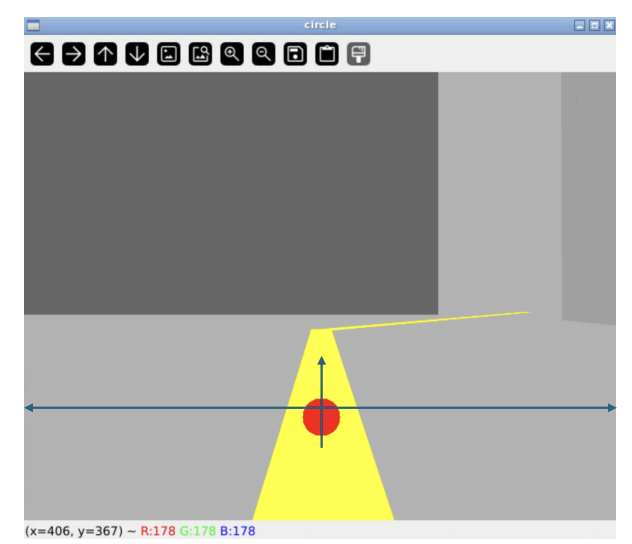
\includegraphics[width=0.7\textwidth]{5.png}
  \caption{Centroid Calculation}
\end{figure}

\section{Motion Control Implementation}

\subsection{Error Calculation}

To ensure accurate line following, calculate the error between the centroid and image center:

\[
  \text{error} = c_x - \frac{\text{width}}{2}
\]

Where:
\begin{itemize}
  \item $c_x$: detected centroid $x$-coordinate.
  \item $\text{width}$: image width.
  \item $\text{error}$: deviation from center.
\end{itemize}

\begin{figure}[H]
  \centering
  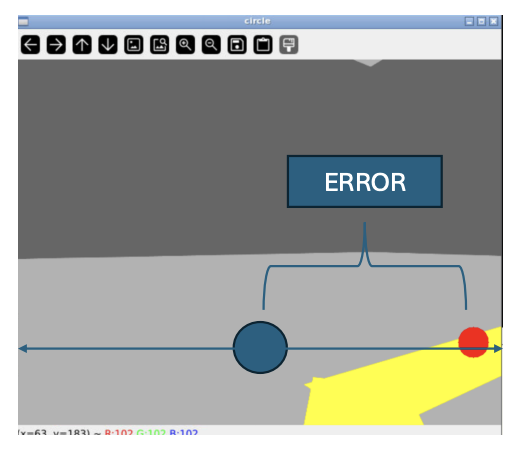
\includegraphics[width=0.75\textwidth]{6.png}
  \caption{Error Calculation}
\end{figure}

\subsection{P Controller}

Based on practical testing, using only a \textbf{P controller} achieves good control results:

\[
  \text{angular\_speed} = -K_p \cdot \text{error}
\]

\paragraph{Notes:}
\begin{itemize}
  \item Simple \textbf{P control} is used instead of full \textbf{PID control}.
  \item Testing showed \textbf{P control alone works better} in this scenario.
  \item Robot response sensitivity can be adjusted through $K_p$ value.
\end{itemize}

\section{Multi-State Decision Implementation}

\subsection{State Definitions}

The system defines three basic states:

\begin{enumerate}
  \item \textbf{State1 (line)}: Yellow line detection state.
  \item \textbf{State2 (obstacle)}: Obstacle detection state.
  \item \textbf{State3 (explore)}: Exploration state.
\end{enumerate}

\subsection{State Transition Logic}

\begin{lstlisting}
if detect_line():
    # Line detected, follow centroid using P control
    follow_centroid()
elif not (detect_line() or detect_obstacle() or is_exploring):
    # No line detected and not exploring, rotate to search
    rotate_search()
    if search_timeout():
        set_explore_mode(True)
elif not (detect_line() or detect_obstacle()) and is_exploring:
    # Exploration mode, move forward to find target
    move_forward()
else:
    # Obstacle encountered, use left-hand rule for avoidance
    left_wall_follower()
\end{lstlisting}

\section{System Limitations and Future Work}

\subsection{Current Limitations}

\paragraph{Color Recognition Limitations}
\begin{itemize}
  \item Only supports \textbf{specific color line} detection.
  \item Challenges with \textbf{multi-colored lines} or actual roads.
\end{itemize}

\paragraph{Obstacle Avoidance Constraints}
\begin{itemize}
  \item May \textbf{lose original line} during avoidance.
  \item Lacks \textbf{line memory} and \textbf{relocation capabilities}.
\end{itemize}

\subsection{Future Improvements}

\begin{itemize}
  \item Introduce \textbf{deep learning methods} to enhance line recognition.
  \item Integrate \textbf{machine learning algorithms} to optimize decision system.
  \item Add \textbf{reinforcement learning} for smarter path planning.
  \item Develop \textbf{more reliable line detection and following algorithms}.
\end{itemize}

\end{document}
